\chapter{\textcolor{myred}{Ecuaciones de Campo de Einstein}}

\newthought{La validez} de la teoría gravitacional de Newton es indiscutible. Sobre las bases de esta teoría podemos determinar el movimiento de planetas, satélites, naves espaciales y hasta fuimos capaces de predecir la existencia de planetas\footnote{Urbain Le Verrier en 1846 predijo la existencia Neptuno debido a unas inconsistencias observadas en la órbita de Urano, usando las leyes de Kepler y Newton. Años más tarde, tal vez sugestionado por su descubrimiento anterior, Le Verrier interpretó que la anomalía en la órbita de Mercurio era debido a un planeta no descubierto que llamo Vulcano. Esto se vio reforzado por un astrónomo que creyó haberlo visto en su telescopio cuando en realidad solo vió una mancha en el lente.}.
De esta manera, a pesar que la teoría gravitacional de Newton entra en conflicto con el principio de equivalencia y las leyes de conservación del momento, la validez esencial de la teoría fue establecida y aceptada durante muchos años. Antes que pensar que la teoría está mal o es incorrecta, porque además, qué está bien o qué mal, está sujeto al contexto y a los conocimientos presentes en un determinado momento de la historia. La verdad no es un absoluto, si no, un acuerdo o consenso entre las personas y esto conlleva a muchas limitaciones. En otras palabras la teoría de Newton es un modelo que sirve para describir gran cantidad de fenómenos de la naturaleza y de forma perfectamente válida, no obstante es plausible que la dicha teoría esté incompleta y necesite ser más desarrollada. En particular, debe ser reformulada de manera tal que cumpla con el principio de equivalencia y satisfaga las leyes de conservación del momento.

\newthought{El objetivo de este capítulo} es construir las ecuaciones tensoriales que describan de una vez por todas los campos gravitatorios. Para ello, comencemos pensando en la \textbf{Ley de Gauss} para el Electromagnetismo, que conecta el campo eléctrico $\mathbf{E}$ con la densidad de carga $\rho$:
    $$\nabla \cdot \mathbf{E}= 4\pi k \rho$$
Cuando desarrolló su Teoría de Gravitación Universal, Newton no contaba con el concepto de campo, pero hoy en día podemos construir un análogo a la Ley de Gauss, para el campo gravitatorio $\mathbf{g}=-\nabla \Phi$ (donde $\Phi$ es el \textbf{potencial gravitatorio}), y una densidad de masa $\rho$:
    $$-\nabla \cdot \mathbf{g}= 4\pi G \rho \hspace{0.5cm}\Longrightarrow\hspace{0.5cm} \nabla^2\Phi=4\pi G\rho$$
Esta ecuación ya tiene una característica favorable: es una \textbf{ecuación de campo local}, es decir que relaciona la derivada del campo con su fuente \textit{en el mismo punto}. Esto nos ahorra el problema de señales instantáneas que presentamos al principio, y también nos permite considerar sistemas localmente inerciales, algo a lo que ya deberíamos estar acostumbradxs. 

Nuestro objetivo será entonces generalizar esta última ecuación. En base a lo que hemos estudiado, podemos anticipar que tendrá esta forma:

\begin{figure}[h!]
    \centering
    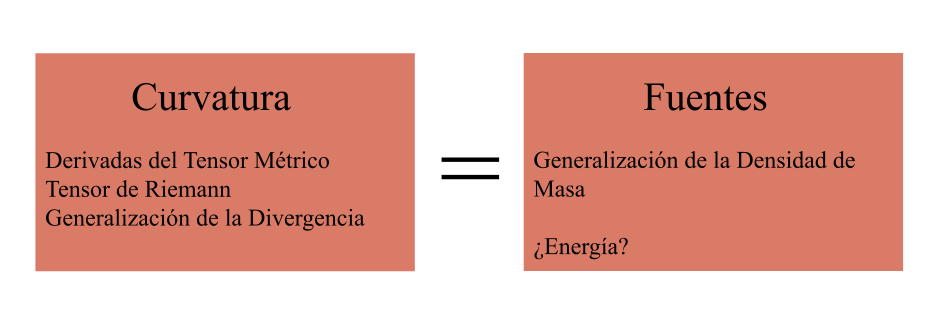
\includegraphics[width=0.95\textwidth]{Im/eceinstein.png}
    \label{fig:sen}
\end{figure}

\newpage
\section{\huge{Tensor de Estrés-Energía}}
\textcolor{myred}{\hrule}
\begin{flushright}
\textit{Anxiety is a scalar,\\fear is a vector,\\stress is a tensor.\\\textbf{Elon Musk} (War Criminal)}
\end{flushright}
El objetivo de esta sección es generalizar la densidad de masa escalar $\rho$ a una magnitud tensorial. Es decir, vamos a trabajar con el lado derecho de la ecuación, las \textit{fuentes}.

\vspace{0.5cm}

Primero podríamos preguntarnos, ¿en la ecuación newtoniana, la densidad $\rho$ representa la masa de un objeto, o es en realidad su \textbf{energía relativista}? En el límite newtoniano, estas dos magnitudes son equivalentes. Se puede demostrar (algo que no haremos aquí), que si la fuente del campo fuera la masa, podríamos crear energía \textit{de la nada}, mientras que 
si consideramos la energía como fuente de la gravedad, esto no sucede.

\vspace{0.25cm}

Lo siguiente sería pensar si $\rho$ pudiera ser una de las entradas de un tensor, de la misma manera que la densidad de carga $\rho$ resultó ser la componente temporal $J^{0}$ de el cuadrivector densidad de corriente $\mathbf{J}$. A este último resultado (propio de la Relatividad Especial), se llega mediante la \textbf{conservación de la carga}, así que podríamos esperar llegar a algo similar aquí apelando a la \textbf{conservación de la energía}.

La construcción de este tensor no es nada trivial, y puede visualizarse mejor mediante ejemplos: la energía-momento del \textbf{polvo} (partícula que se mueven estando en reposo unas respecto de las otras), o la energía-momento de un \textbf{fluido perfecto} (un conjunto de partículas que se mueven aleatoriamente pero no interactúan entre sí, por ejemplo un gas ideal). Vamos a pasar por alto estos ejemplos y caer directamente en el tensor, explicando sus componentes y sus propiedades:
\begin{remarkbox}{Tensor de Estrés-Energía o Energía-Momento}
    \centering
    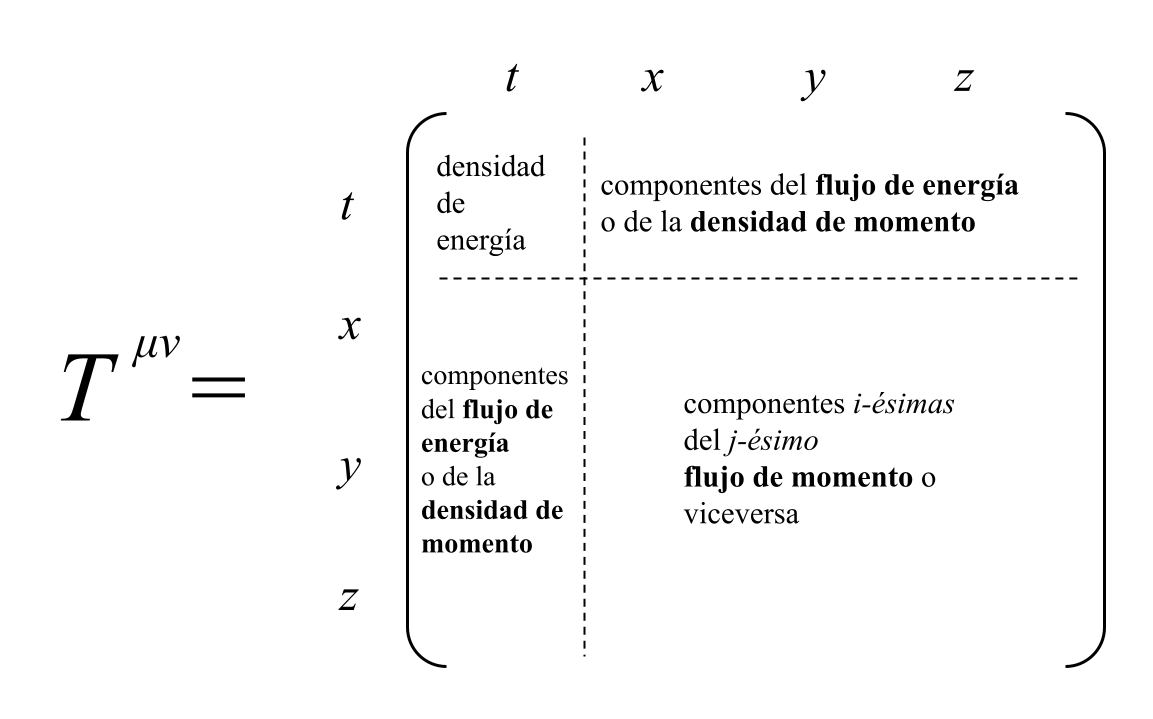
\includegraphics[width=0.85\textwidth]{Im/tensor.png}
\end{remarkbox}

De este tensor vamos a enunciar las siguientes propiedades:
\begin{itemize}
    \item Es \textbf{simétrico}, es decir que:
    $$T^{\mu\nu}=T^{\nu\mu}$$
    \item La \textbf{conservación de energía y flujo de momento} nos garantizan que:
    $$\nabla_{\nu}T^{\mu\nu}=0$$
\end{itemize}

Como vamos a estudiar la ecuación de campo de un agujero negro con carga eléctrica (Reissner-Nordström), vamos a buscar el tensor de estrés energía para un campo electromagnético.

\begin{remarkbox}{Tensor de Estrés-Energía Electromagnético}

    Recordemos primero el \textbf{tensor de campo electromagnético} $F^{\mu\nu}$:
    \begin{equation}
    F_{\alpha\beta}=
    \begin{pmatrix}
    0 & E_1/c & E_2/c & E_3/c\\
    -E_1/c & 0 & -B_3 & B_2\\
    -E_2/c & B_3 & 0 & -B_1\\
    -E_3/c & -B_2 & B_1 & 0
    \end{pmatrix}
    \label{tensorcampoelectromagnetico}
    \end{equation}

    Sabemos además que, para un campo EM, la \textbf{densidad de energía} está dada por:
    $$\rho_E=\frac{1}{2\mu_0}\left(E^2+B^2\right)$$
    
    Como los campos EM almacenan energía, tienen que tener un tensor de stress-energía asociado. Los únicos elementos que intervienen aquí son los campos electromagnéticos y el espacio-tiempo, por lo que $T^{\mu\nu}$ (simétrico) deberá ser una combinación de $F^{\mu\nu}$ (antisimétrico) y $g_{\mu\nu}$ (simétrico). Tomando esto en cuenta, y además pidiendo que la entrada $tt$ corresponda a la densidad de energía $\rho_E$ de más arriba, podemos llegar al siguiente tensor:
    \begin{equation}
    T^{\mu\nu}=\frac{1}{\mu_0}\left(\frac{1}{4}g^{\mu\nu}F^{\sigma\gamma}F_{\sigma\gamma}-F^{\mu\alpha}g_{\alpha\beta}F^{\nu\beta}\right)
    \label{tensorestresenergiafunciondeF}
    \end{equation}
    
    
    Una característica destacable de este tensor es que es \textbf{traceless} (traza nula). Es decir que, si bajamos un índice y contraemos, podemos demostrar que:
    
    \begin{equation}
        T\equiv T^{\alpha}_{\alpha}=0
        \label{traceless}
    \end{equation}
\end{remarkbox}

\newpage

\section{\huge{Ecuaciones de Campo de Einstein}}

\textcolor{myred}{\hrule}

\newthought{Ya obtuvimos} lo que va al lado derecho de las ecuaciones de campo. Lo que nos queda por hacer es construir el lado izquierdo de la misma. Evidentemente, el dado izquierdo también deberá:

\begin{itemize}
    \item Ser un \textbf{tensor contravariante de segundo rango}, al que llamaremos $G^{\mu\nu}$, tal que:
    
    $$G^{\mu\nu}=k T^{\mu\nu}$$
    
    ($k$ es una constante de proporcionalidad a determinar).
    
    \item Ser \textbf{simétrico}, es decir que $G^{\mu\nu}=G^{\nu\mu}$.
    \item Tener \textbf{gradiente absoluto nulo}, es decir $\nabla_{\mu}G^{\mu\nu}=0.$
    \item Representar la \textbf{curvatura} del espacio-tiempo, es decir que deberá \textbf{contener derivadas segundas del tensor métrico} $g_{\mu\nu}$.
    \item Reducirse a la fórmula newtoniana $\nabla^2\Phi=4\pi G \rho$ en el límite no-relativista.
\end{itemize}

Una primer propuesta que podríamos hacer es utilizar el \textbf{tensor de Ricci} (que, si recordamos, era una contracción del tensor de Riemann, el cual contiene toda la información necesaria para describir la curvatura del espacio-tiempo). Si bien este tensor es simétrico, el problema yace en que, en general, $\nabla_\mu R^{\mu\nu}\neq0$, por lo que tendremos que proponer algo distinto.

\vspace{0.5cm}

¿Qué otras cosas podemos agregar? Los únicos elementos razonables podrían ser otras contracciones del tensor de Riemann (por ejemplo, el escalar de curvatura $R$), y el propio tensor métrico $g^{\mu\nu}$. La forma más general de combinar esto (respetando el requisito de simetría) es la siguiente:

$$G^{\mu\nu}=R^{\mu\nu}+b g^{\mu\nu} R+\Lambda g^{\mu\nu}$$

Donde $b$ y $\Lambda$ son constantes (escalares).

Si pedimos que, además, $\nabla_{\nu}G^{\mu\nu}=0$, tenemos que:

\begin{equation}
\begin{split}
\nabla_{\nu}G^{\mu\nu}&=\nabla_{\nu}\left(R^{\mu\nu}+b g^{\mu\nu} R+\Lambda g^{\mu\nu}\right)=\\
&=\nabla_{\nu}\left(R^{\mu\nu}+b g^{\mu\nu} R\right)=0
\end{split}
\end{equation}

\begin{marginfigure}
\begin{remarkbox}{Identidad de Bianchi}
$$\nabla_\sigma R_{\alpha\beta\mu\nu}+\nabla_\nu R_{\alpha\beta\sigma\mu}+$$ $$\nabla_\mu R_{\alpha\beta\nu\sigma}=0$$
\end{remarkbox}
\end{marginfigure}

Si utilizamos la \textbf{identidad de Bianchi}, podemos demostrar que es necesario que $b=-\frac{1}{2}$. La ecuación toma entonces la forma:

\begin{equation}
    R^{\mu\nu}-\frac{1}{2} g^{\mu\nu} R+\Lambda g^{\mu\nu}=k T^{\mu\nu}
\end{equation}

Podemos utilizar ahora el requisito de que la ecuación se reduzca a la newtoniana en el límite no-relativista para determinar el valor de la constante $k$. Esto consiste en considerar el \textbf{límite de campo débil}\cite[][p.255]{moore}, e implementar las desviaciones geodésicas. Nos saltearemos esta deducción\cite[][p.246]{moore} para concluir que es necesario que $k=8\pi G$. Las ecuaciones de campo son entonces:

\begin{marginfigure}
\begin{remarkbox}{Weak-Field Limit}
El \textbf{Límite de Campo Débil} consiste en proponer un tensor métrico que difiere muy levemente del $\eta_{\mu\nu}$ del espacio de Minkowski. Es posible demostrar, mediante un análisis perturbativo, que en dicho límite la entrada $g_{00}$ del tensor métrico tiene la forma:

\begin{equation}
    g_{00}=1-\frac{2GM}{c^2 r}
    \label{g00}
\end{equation}

Que está íntimamente relacionada con el potencial gravitatorio newtoniano.
\end{remarkbox}
\end{marginfigure}

\begin{remarkbox}{Ecuaciones de Campo de Einstein}
\begin{equation}
    R^{\mu\nu}-\frac{1}{2} g^{\mu\nu} R+\Lambda g^{\mu\nu}=8 \pi G T^{\mu\nu}
\end{equation}
\end{remarkbox}

La constante $\Lambda$ se llama \textbf{constante cosmológica}, y en los análisis posteriores podemos considerarla igual a cero.

Multiplicando por el tensor métrico y contrayendo un par de índices, podemos llegar a una forma alternativa para las ecuaciones:

\begin{remarkbox}{Ecuaciones de Campo de Einstein - Forma Alternativa}
\begin{equation}
    R^{\mu\nu}=8 \pi G\left(T^{\mu\nu}-\frac{1}{2} g^{\mu\nu} T\right)+\Lambda g^{\mu\nu}
    \label{campoeinsteincontravariante}
\end{equation}
\end{remarkbox}

\newpage

\section{\huge{Geodésicas}}
\textcolor{myred}{\hrule}
\begin{flushright}
\textit{It took the light,\\ absolutely forever to get to your eyes.\\\textbf{Alex Turner}}
\end{flushright}

\newthought{Ya sabemos a la perfección cómo es que la energía modifica la geometría del espacio-tiempo}. Lo que nos queda por explicar ahora es cómo un objeto se mueve en este espacio-tiempo curvado, para poder hallar ecuaciones diferenciales de movimiento. 

Para esto, vamos a definir una \textbf{geodésica} como la \textbf{curva entre dos eventos con el mayor tiempo propio}. La hipótesis geodésica dice que, en los espacio-tiempos con cualquier tipo de geometría (incluso curvados), los cuerpos libres de fuerzas se mueven en geodésicas. Es decir que, al viajar de un punto $A$ a un punto $B$ en el espacio-tiempo, de todas las posibles trayectorias los cuerpos 'eligen' la que hace que sus relojes midan más tiempo propio.

Veamos qué se puede hacer con esta hipótesis.

\subsection*{\textbf{Geodésicas Timelike}}

\begin{marginfigure}
\captionsetup{type=figure}
    \centering
    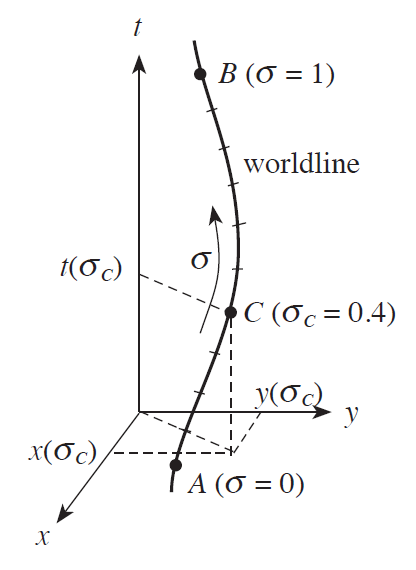
\includegraphics[width=1.3\textwidth]{Im/geod.png}
    \caption{Podemos describir la curva (worldline) entre dos eventos $A$ y $B$ etiquetando todos los eventos entre ellos mediante un parámetro $\sigma$, luego especificando las coordenadas espaciales y temporales de dichos eventos como función de dicho parámetro.}
    \label{fig:sen}
\end{marginfigure}

Tomemos dos eventos $A$ y $B$ que tienen una separación de tipo \textit{timelike} (es decir con $ds^2>0$, el movimiento de las partículas con masa, que viajan a velocidades inferiores a la de la luz). Pensemos en las posibles trayectorias que conectan los dos eventos, y hagámoslas variar con un parámetro $\sigma$, que va de $0$ a $1$. Es decir, vamos a especificar $x^{\mu}(\sigma)$ a lo largo de la trayectoria. El tiempo propio a lo largo de esta trayectoria va a estar dado por:

\begin{equation}
    \tau_{AB}=\int \sqrt{-ds^2}=\int_0^1\sqrt{-g_{\mu\nu}(x^{\alpha}(\sigma))\frac{dx^\mu}{d\sigma}\frac{dx^\nu}{d\sigma}}d\sigma
\end{equation}

Hallar la curva que maximice el valor de $\tau_{AB}$ es muy similar a cuando, en Mecánica Clásica, buscamos la trayectoria $q_i(t)$ que \textbf{minimice la acción $S$}, la cual estaba definida como:

$$S\equiv \int_{t_a}^{t_b}L(q_i,\Dot{q}_i)dt$$

Donde $L$ es el \textbf{lagrangiano} del sistema, una función de las coordenadas generalizadas y las velocidades generalizadas. A partir de este principio variacional, llegábamos a las \textbf{Ecuaciones de Euler-Lagrange}:

\begin{equation}
    \frac{d }{dt}\left(\frac{\partial L}{\partial \dot{q}_i}\right)-\frac{\partial L}{\partial q_i}=0
\end{equation}

La situación aquí es completamente análoga. Podemos armar un lagrangiano que depende de las posiciones $x^{\mu}$ y las 'velocidades' $\dot{x}^\mu \equiv d x^\mu / d\sigma$:

\begin{remarkbox}{Lagrangiano}
\begin{equation}
    L(x^{\alpha},\dot{x}^{\alpha})\equiv\sqrt{-g_{\mu\nu}(x^{\alpha})\dot{x}^{\mu}\dot{x}^{\nu}}
\end{equation}
\end{remarkbox}

Que, de igual manera, nos conducen a las ecuaciones:

\begin{remarkbox}{Ecuaciones de Euler-Lagrange}
\begin{equation}
    \frac{d }{d\sigma}\left(\frac{\partial L}{\partial \dot{x}^{\alpha}}\right)-\frac{\partial L}{\partial x^{\alpha}}=0
\end{equation}
\end{remarkbox}

Se puede proceder reemplazando el lagrangiano y derivando, y luego de un buen trabajo algebraico, llegamos a la siguiente ecuación:

\begin{remarkbox}{Ecuación geodésica}
\begin{equation}
\frac{d}{d\tau}\left(g_{\alpha\beta}\frac{dx^{\beta}}{d\tau}\right)-\frac{1}{2}\partial_\alpha g_{\mu\nu}\frac{dx^{\mu}}{d\tau}\frac{dx^{\nu}}{d\tau}=0
\end{equation}
\end{remarkbox}

Esta ecuación es muy conveniente, ya que utiliza el tensor métrico de forma explícita, en lugar de tenerlo 'oculto' en el lagrangiano. También nos hemos independizado del parámetro $\sigma$, aunque a veces nos será conveniente volver a dicho parámetro arbitrario, como es en el caso de las geodésicas \textit{lightlike}, es decir la trayectoria de fotones. Para cualquier trayectoria, el $\tau_{AB}$ de la luz es siempre cero (podríamos decir que \textit{un reloj moviéndose a la velocidad de la luz no avanza}), por lo que $\tau$ deja de ser un buen parámetro.

También es posible utilizar los \textbf{símbolos de Christoffel} para reescribir la ecuación geodésica. Esta se lee:

\begin{remarkbox}{Ecuación geodésica - Forma Alternativa}
\begin{equation}
\frac{d^2x^{\mu}}{d\tau^2}+\Gamma^{\mu}_{\alpha\beta}\frac{dx^{\alpha}}{d\tau}\frac{dx^{\beta}}{d\tau}=0
\label{geodesicx}
\end{equation}
\end{remarkbox}

\begin{figure}
    \centering
    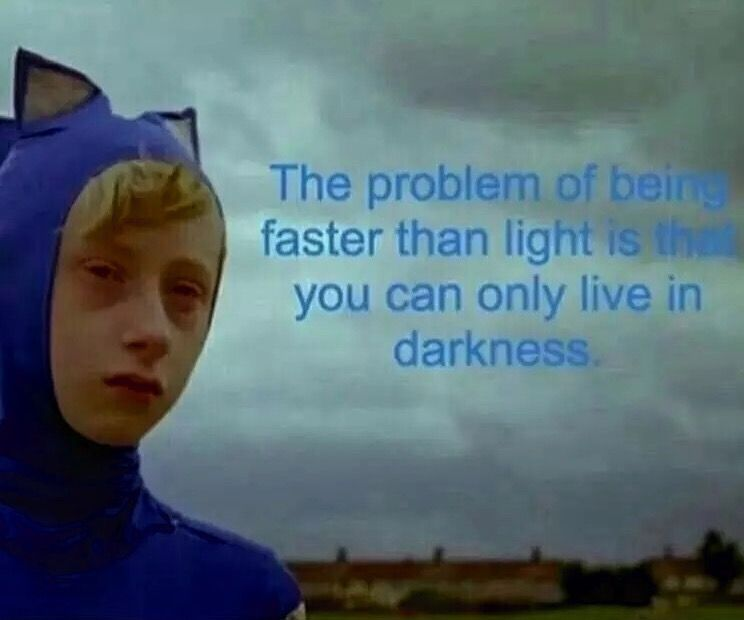
\includegraphics[width=0.6\textwidth]{Im/sonic.jpg}
    \caption{El único meme que pusimos en este trabajo.}
    \label{fig:my_label}
\end{figure}






